\documentclass[12pt, letterpaper, oneside]{article}
\usepackage[nolinks]{qrcode}
\usepackage[absolute,overlay]{textpos}
\usepackage[letterpaper,  left=30mm, right = 30mm, top=40mm, bottom=20mm]{geometry}                		
\usepackage{graphicx}
\usepackage{tikz}
\usetikzlibrary{calc,through,intersections, arrows, shapes, decorations.markings, matrix, patterns}
\usepackage{enumitem}

\usepackage{pdfpages}
\usepackage{amsmath,amssymb,amscd,amsthm,eucal,curves,epic, graphicx}
\usepackage[all]{xy}
\usepackage{color}
\usepackage{hyperref}
\usepackage{rotating}
\usepackage{enumitem}

%---------------------------------------------------
% TiKZ
%---------------------------------------------------
\usepackage{tikz}
\usetikzlibrary{calc,through,intersections, arrows, shapes, matrix, patterns, calligraphy, positioning}
\usetikzlibrary{decorations.pathmorphing, decorations.markings}
\usepackage{tikz-3dplot}
\usetikzlibrary{arrows.meta}
\usetikzlibrary{bending}
\usepackage{pgf, pgfplots}
\usepgflibrary{plotmarks}
\pgfplotsset{compat=1.12}
\tikzset{>=latex}

\newcommand{\btikz}[1][]{\begin{equation*}\begin{tikzpicture}[#1]}
\newcommand{\etikz}{\end{tikzpicture}\end{equation*}}


%---------------------------------------------------
% Colors
%---------------------------------------------------
\definecolor{myblue}{rgb}{0,.25,.6}
\definecolor{light}{gray}{.95}
\definecolor{lines}{RGB}{60, 60, 60}
\definecolor{shadecolor}{rgb}{.95,1,1}



%---------------------------------------------------
% Fonts
%---------------------------------------------------
\usepackage{pifont}
\usepackage[math]{iwona}



\newcount\problemCount %% problem counter
\problemCount=1
\newcount\subproblemCount %% subproblem counter
\subproblemCount=97 %% 97 = the ascii character code for 'a'


\thispagestyle{empty}

\newcommand{\brk}{\vfill\eject}

%% \prob resets \subprobCount, typesets problem number according to 
%% \probCounter value and advances \probCounter. 
\newcommand{\prob}[1][]{\subproblemCount=97\noindent{\bf {\number\problemCount}{{\bf #1}}. }\advance\problemCount by 1}


%% \subprobCount typesets subproblem number according to 
%% \subprobCounter value and advances \subprobCount
\newcommand{\subprob}{\par\vskip.2cm\noindent{\bf\char\subproblemCount ) }\advance\subproblemCount by 1}

%% \subprobns is a variant of \subprob which does not skip 
%% vertical space before typesetting the subproblem number.
\newcommand{\subprobns}{\noindent{\bf\char\subproblemCount ) }\advance\subproblemCount by 1}




%Vectors
\newcommand{\bb}{\mathbf b}
\newcommand{\be}{\mathbf e}
\newcommand{\bn}{\mathbf n}
\newcommand{\bu}{\mathbf u}
\newcommand{\bv}{\mathbf v}
\newcommand{\bw}{\mathbf w}
\newcommand{\by}{\mathbf y}
\newcommand{\bx}{\mathbf x}
\newcommand{\bz}{\mathbf z}
\newcommand{\bzero}{\mathbf 0}

%Varia
\newcommand{\ra}{\rightarrow}
\newcommand{\bbm}{\begin{bmatrix}}
\newcommand{\ebm}{\end{bmatrix}}

\newcommand{\msp}{\phantom{-}}



\renewcommand{\H}{\mathbb{H}}
\newcommand{\C}{\mathbb{C}}
\newcommand{\R}{\mathbb{R}}
\newcommand{\Q}{\mathbb{Q}}
\newcommand{\Z}{\mathbb{Z}}
\newcommand{\fd}{\mathbb{F}}



\DeclareMathOperator{\Span}{Span}
\DeclareMathOperator{\col}{Col}
\DeclareMathOperator{\Nul}{Nul}
\DeclareMathOperator{\row}{Row}
\DeclareMathOperator{\adj}{adj}
\DeclareMathOperator{\area}{area}
\DeclareMathOperator{\Ker}{Ker}
\DeclareMathOperator{\im}{Im}
\DeclareMathOperator{\rank}{rank}
\DeclareMathOperator{\dist}{dist}
\DeclareMathOperator{\proj}{proj}





\renewcommand{\geq}{\geqslant}
\renewcommand{\leq}{\leqslant}

%\usepackage[math]{iwona}


%%%%%%%%%%%%%%%%%%%%%%%%%%%%
%   END MACROS
%%%%%%%%%%%%%%%%%%%%%%%%%%%%


\begin{document} 

\thispagestyle{empty}

%---------------------------------------------------
%  TITLE PAGE
%---------------------------------------------------


\thispagestyle{empty}
\newgeometry{left=10mm, right=10mm, top=40mm, bottom=20mm} 

\ 

\begin{center}
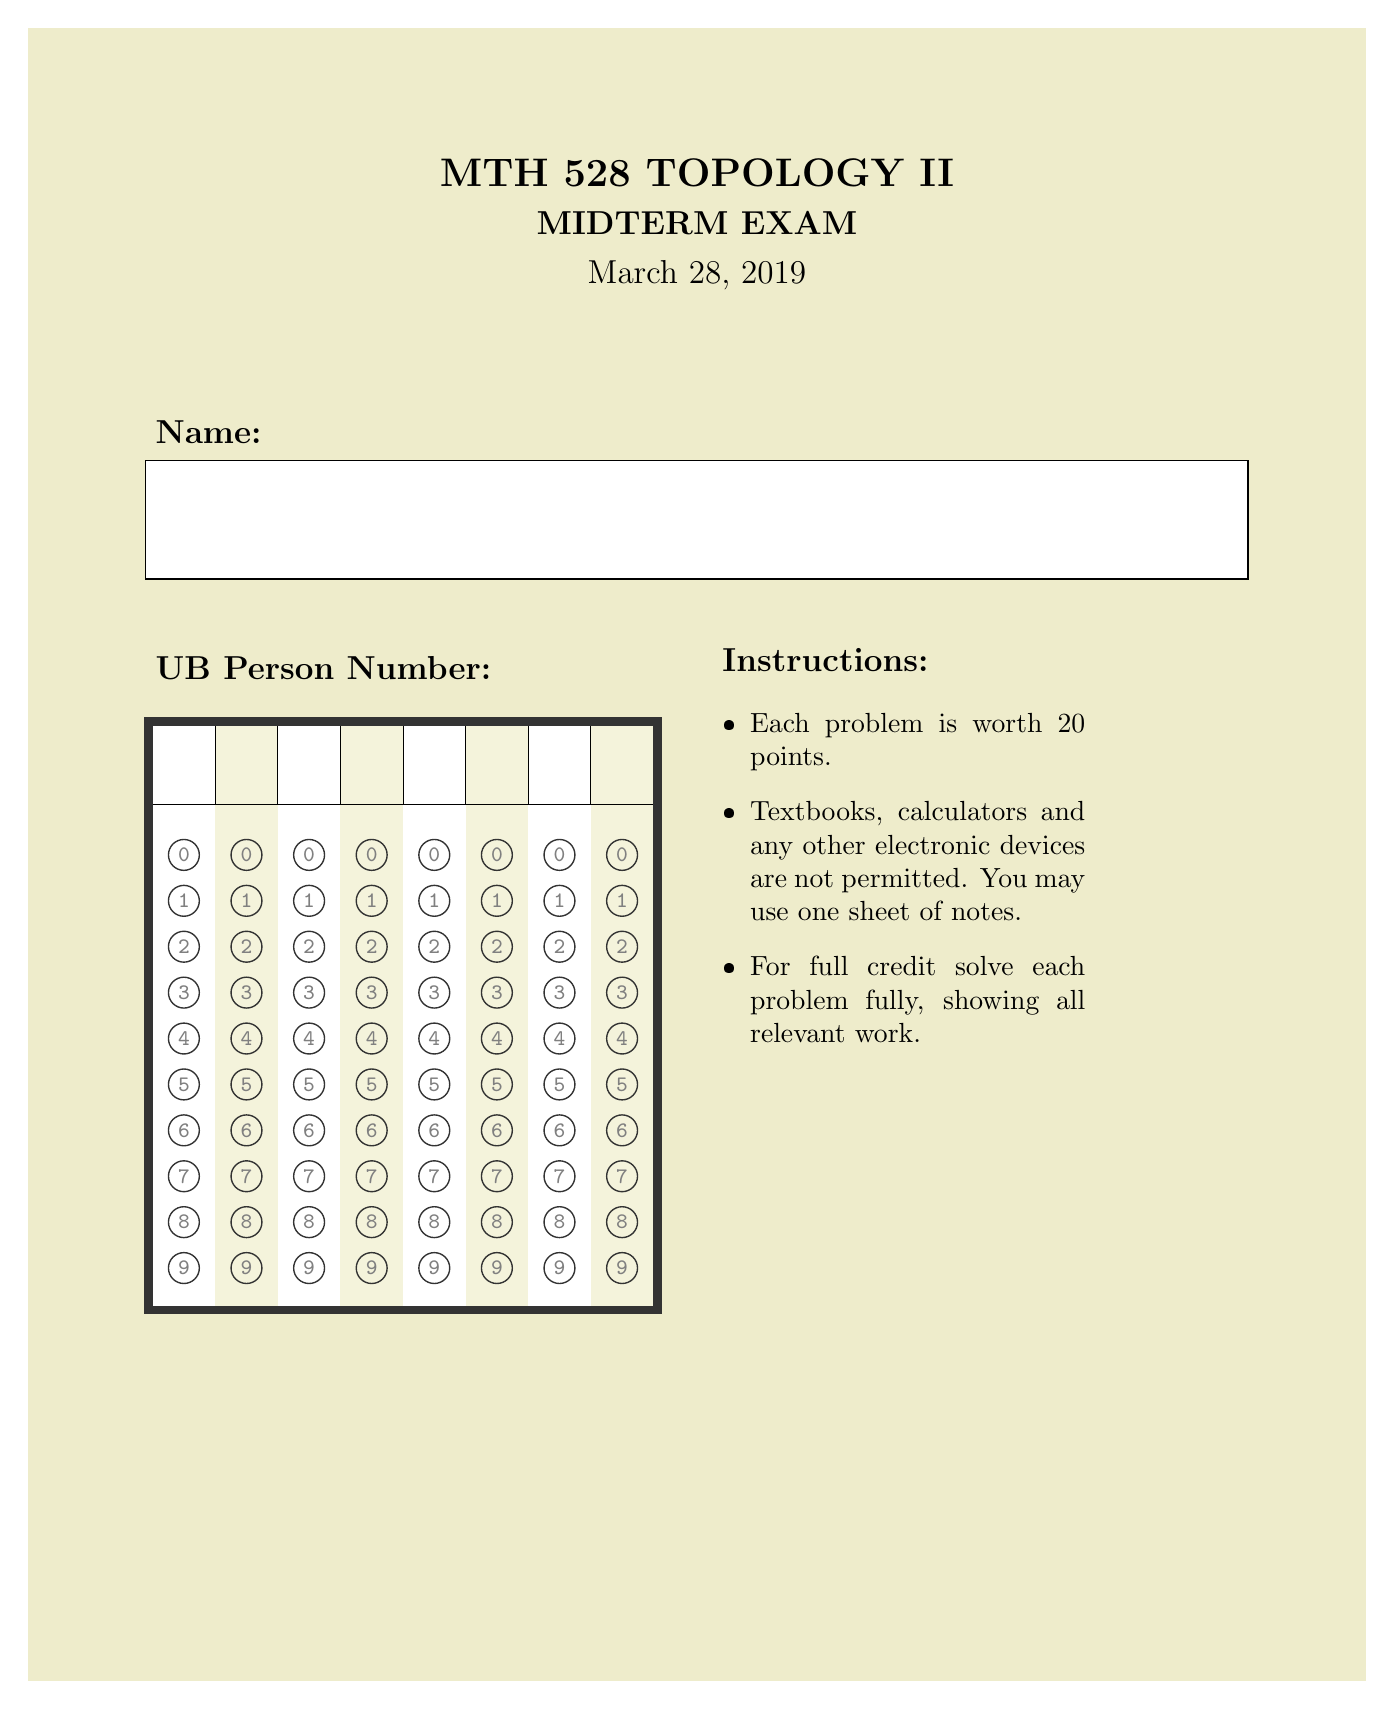
\begin{tikzpicture}
%background and header
\fill[olive!15] (-0.5,0) rectangle (16.5, 21);
\node at (8, 18.5) {\begin{minipage}{\textwidth}
\begin{center}
{\Large \bf{MTH 528 TOPOLOGY II}}\\[2mm]
{\large \bf{MIDTERM EXAM}} \\[2mm]
 {\large March 28, 2019} \\
\end{center}
\end{minipage}
};

% name box
\node[anchor = south west] at (1, 15.6) {\large \bf Name:};
\draw[fill  = white, line width = 0.5]  (1, 14) rectangle +(14, 1.5);



% person number
\node[anchor = south west] at (1, 12.6) {\large \bf UB Person Number:};

\begin{scope}[scale=0.53, yshift = 200mm, xshift =13mm]
\draw[black!50, fill = white, line width = 3]  (0.65, 3) rectangle +(8*1.5 + 0.2, -1.1*11-2);

\foreach \x in {1,3,5,7}{
\fill[olive!10]  (0.75 + 1.5*\x, 3) rectangle +(1.5, -1.1*11 - 2);
};
\foreach \x in {1,...,8}{
\draw[line width = 0.3]  (1.5*\x-0.75, 1) rectangle +(1.5, 2);
}

\draw[black!80,  line width = 3]  (0.65, 3) rectangle +(8*1.5 + 0.2, -1.1*11-2);

\foreach \y [evaluate={\z=int(-1*\y);}] in {0,-1,...,-9}{
\foreach \x in {1,...,8}{
\draw[line width = 0.5, color=black!80 ] (1.5*\x, 1.1*\y- 0.2) circle (0.37);
\node at (1.5*\x, 1.1*\y - 0.2) {\footnotesize \color{black!50}\tt \z};
};
}
\end{scope}



% instructions
\node[anchor=north west] at (8.2, 13.24) {\begin{minipage}{0.38\textwidth}
{\large \bf Instructions:}


\begin{itemize}[leftmargin=*]
\item  Each problem is worth 20 points. 

\item Textbooks, calculators and any other electronic devices are not permitted. 
You may use one sheet of notes.  

\item For full credit solve each problem fully, showing all relevant work.
\end{itemize}  

\end{minipage}
};


\end{tikzpicture}
\end{center}

%% QR CODE
\begin{textblock*}{11cm}[1, 0](8.2in, 0.3in) % {block width} [anchor point] (coords) 

\begin{tikzpicture}
\draw[opacity = 0] (-8, 0) rectangle (2.2 , -2.2);
\node[fill=white, anchor= north west] at (0,0)
{\qrcode[height=25mm, level=H]{MTH-309T-F19-EX1-005-P00}};
\node[anchor =  north east] at (0, -1) {\large\tt \begin{tabular}{r} MTH-309T-F19-EX1-005-P00 \end{tabular}};
\end{tikzpicture}
\end{textblock*}
%% END QR CODE


\restoregeometry

%---------------------------------------------------
% END TITLE PAGE
%---------------------------------------------------


\newpage 




%% QR CODE
\begin{textblock*}{11cm}[1, 0](8.2in, 0.3in) % {block width} [anchor point] (coords) 

\begin{tikzpicture}
\draw[opacity = 0] (-8, 0) rectangle (2.2 , -2.2);
\node[fill=white, anchor= north west] at (0,0)
{\qrcode[height=25mm, level=H]{MTH-309T-F19-EX1-005-P01}};
\node[anchor =  north east] at (0, -1) {\large\tt \begin{tabular}{r} MTH-309T-F19-EX1-005-P01 \end{tabular}};
\end{tikzpicture}
\end{textblock*}
%% END QR CODE

\prob Let $A$ be a matrix and  $\bv$ be a vector given as follows:
$$
A=
\bbm
\  1 & 1 & 1 & 1 \ \\
\  0 & 0 & 1 & 1 \ \\
\  0 & 0 & 1 & 1 \ \\
\  0 & 0 & 0 & 0 \ \\
\ebm
\hskip 8mm
\bv = 
\bbm
\msp 1\  \\
-1\  \\
-1\  \\
\msp 1\  \\
\ebm 
$$

\subprob Determine if $\bv$ is in $\col(A)$, where $\col(A)$ is the column space of $A$.

\subprob Determine if $\bv$ is in $\Nul(A)$, where $\Nul(A)$ is the null space of $A$. 

\subprob Find an explicit description of $\Nul(A)$ by listing vectors that span the null space. 




\brk


%% QR CODE
\begin{textblock*}{11cm}[1, 0](8.2in, 0.3in) % {block width} [anchor point] (coords) 

\begin{tikzpicture}
\draw[opacity = 0] (-8, 0) rectangle (2.2 , -2.2);
\node[fill=white, anchor= north west] at (0,0)
{\qrcode[height=25mm, level=H]{MTH-309T-F19-EX1-005-P01}};
\node[anchor =  north east] at (0, -1) {\large\tt \begin{tabular}{r} MTH-309T-F19-EX1-005-P01 \end{tabular}};
\end{tikzpicture}
\end{textblock*}
%% END QR CODE



\prob Consider the following matrices:


$$B = 
\bbm
\  0  &\  1  &\ 1 \      \cr
\  0  &\  1  &\  0  \    \cr
\  1  &\  0   &\  1 \   \cr
\ebm
\hskip 8mm
C= 
\bbm
\  0 & \ 2 & \ 1 \   \\
\  1 &  \  0 & \ 3 \  \\
\  0 & \  2 & \ 2 \ \\
\ebm
\hskip 8mm
$$

\subprob Compute the inverse of $B$. 

\subprob Find the matrix $A$ such that $(BA)^{T}= C$. 

\brk



%% QR CODE
\begin{textblock*}{11cm}[1, 0](8.2in, 0.3in) % {block width} [anchor point] (coords) 

\begin{tikzpicture}
\draw[opacity = 0] (-8, 0) rectangle (2.2 , -2.2);
\node[fill=white, anchor= north west] at (0,0)
{\qrcode[height=25mm, level=H]{MTH-309T-F19-EX1-005-P01}};
\node[anchor =  north east] at (0, -1) {\large\tt \begin{tabular}{r} MTH-309T-F19-EX1-005-P01 \end{tabular}};
\end{tikzpicture}
\end{textblock*}
%% END QR CODE


\prob Let $T\colon \R^{2}\to \R^{2}$ be the linear transformation which first 
reflects points through the line $x_{1}=x_{2}$ and then reflects points through 
the  $x_{1}$-axis.

\vskip 5mm 

\subprob Find the standard $A$ matrix of $T$. 

\vskip 5mm 

\subprob Find all vectors $\bv\in \R^{2}$ such that $\bv\in \Nul(A)$.

\brk


%% QR CODE
\begin{textblock*}{11cm}[1, 0](8.2in, 0.3in) % {block width} [anchor point] (coords) 

\begin{tikzpicture}
\draw[opacity = 0] (-8, 0) rectangle (2.2 , -2.2);
\node[fill=white, anchor= north west] at (0,0)
{\qrcode[height=25mm, level=H]{MTH-309T-F19-EX1-005-P01}};
\node[anchor =  north east] at (0, -1) {\large\tt \begin{tabular}{r} MTH-309T-F19-EX1-005-P01 \end{tabular}};
\end{tikzpicture}
\end{textblock*}
%% END QR CODE


\prob Consider the following vectors in $\R^{3}$: 
$$
\bv_{1}= 
\bbm
 \msp 1\ \  \cr
 \msp 0\ \ \cr
 \msp 2\ \ \cr
\ebm,\hskip 5mm
\bv_{2}=
\bbm
 -1 \ \ \cr
 \msp 1\ \ \cr
- 2\ \  \cr
 \ebm
 ,\hskip 5mm
\bv_{3}=
\bbm
 \msp 1\ \ \cr
 \msp 2\ \ \cr
 \msp 3\ \ \cr
\ebm
, \hskip 5mm
\bw = 
\bbm
\msp 2\ \ \cr
\msp 2\ \ \cr
\msp b\ \  \cr
\ebm
$$

\subprob Find all values of $b$ such that $\bw\in {\rm Span}(\bv_{1}, \bv_{2}, \bv_{3})$. 

\subprob Let  $b=7$. Express $\bw$ as a linear combination of vectors 
$\bv_{1}$, $\bv_{2}$, $\bv_{3}$.

\subprob Is the set $\{\bv_{1}, \bv_{2}, \bv_{3}\}$ linearly independent? Justify your answer.

\brk

%% QR CODE
\begin{textblock*}{11cm}[1, 0](8.2in, 0.3in) % {block width} [anchor point] (coords) 

\begin{tikzpicture}
\draw[opacity = 0] (-8, 0) rectangle (2.2 , -2.2);
\node[fill=white, anchor= north west] at (0,0)
{\qrcode[height=25mm, level=H]{MTH-309T-F19-EX1-005-P01}};
\node[anchor =  north east] at (0, -1) {\large\tt \begin{tabular}{r} MTH-309T-F19-EX1-005-P01 \end{tabular}};
\end{tikzpicture}
\end{textblock*}
%% END QR CODE


\prob  For each of the statements given below decide if it is true or false. If it is true explain why. 
If it is false give a counterexample. 

\vskip 5mm 

\subprob If $A$, $B$ are $2\times 2$ matrices such that $AB =0$ is the zero matrix (e.i. the matrix with all entries 
equal to zero) then either $A$ or $B$ must be the zero matrix. 

 \vskip 5mm 

\subprob  If $\bu, \bv, \bw$ are vectors in $\R^{3}$ such that the set $\{\bu,\bv, \bw \}$
is linearly independent then the  set $\{\bu, \bv+\bw \}$   must be linearly independent.  

\vskip 5mm 


\subprob If $A$ is a $2\times 2$ matrix and $\bu, \bv$ are vectors in  $\R^{2}$ such that $A\bu$,
$A\bv$ are linearly dependent then  $\bu, \bv$ also must be linearly dependent. 

\vskip 5mm 

\subprob If $T\colon \R^{2} \to \R^{2}$ is a linear transformation and $\bu, \bv, \bw\in \R^{2}$ are 
vectors such that $\bu$ is in $\Span(\bv, \bw)$ then  $\bu$ must be also in $\Span(T(\bv), T(\bw))$. 


\brk 

\end{document}

